\documentclass[11pt,a4paper]{article}

\usepackage[utf8]{inputenc}
\usepackage[T1]{fontenc}
\usepackage[a4paper,margin=1in]{geometry}
\usepackage{amsmath,amssymb,amsfonts}
\usepackage{booktabs,array}
\usepackage{graphicx}
\usepackage{xcolor}
\usepackage{listings}
\usepackage[inline]{enumitem}
\usepackage{hyperref}
\usepackage{setspace}
\usepackage{fancyhdr}
\usepackage{titlesec}
\usepackage{microtype}

\setstretch{1.08}
\setlength{\parindent}{0pt}
\setlength{\parskip}{0.6em}

\pagestyle{fancy}
\fancyhf{}
\setlength{\headheight}{14pt}
\lhead{Assignment 3}
\rhead{Wind Farm Analysis Using FLORIS}
\cfoot{\thepage}

\titleformat{\section}{\large\bfseries}{\thesection.}{0.5em}{}
\titleformat{\subsection}{\normalsize\bfseries}{\thesubsection}{0.5em}{}

\definecolor{codegray}{RGB}{248,248,248}
\definecolor{codeborder}{RGB}{220,220,220}

\lstdefinestyle{mystyle}{
	backgroundcolor=\color{codegray},
	\tframe=single,
	rulecolor=\color{codeborder},
	basicstyle=\ttfamily\small,
	breaklines=true,
	columns=fullflexible,
	keepspaces=true,
	showstringspaces=false,
	tabsize=4
}
%\lstset{style=mystyle}

\title{\textbf{Assignment 3}\\\normalsize Wind Farm Analysis Using FLORIS}
\author{Chinmay S Patil}
\date{}

\graphicspath{{../}}

\begin{document}
	\maketitle
	
	\section{Introduction}
	This assignment studies a small wind farm consisting of three \textbf{IEA 3.4 MW} wind turbines placed in a row with a rotor diameter of $D = 130$ m and a hub height of 120 m. The main goals are to define the turbine in FLORIS, validate its characteristics, visualize wake interactions, compute power output with different wake models, and compare the influence of turbine spacing and atmospheric conditions.
	
	The notebook uses FLORIS together with the turbine data read from the provided CSV file. The turbine is modeled as a pitch-regulated machine with rated power 3370 kW, rated wind speed 9.8 m/s, cut-in wind speed 3 m/s, and cut-out wind speed 25 m/s.
	
	\section{Question 1: Define the turbine in FLORIS}
	The first step was to define the turbine and store it as a FLORIS turbine description. The CSV file was read, and the key rated parameters were used to build the turbine configuration.
	
	\subsection*{Key parameters used}
	\begin{center}
		\begin{tabular}{ll}
			\toprule
			Parameter & Value \\
			\midrule
			Name & IEA 3.4 MW Reference \\
			Rated power & 3370 kW \\
			Rated wind speed & 9.8 m/s \\
			Cut-in wind speed & 3 m/s \\
			Cut-out wind speed & 25 m/s \\
			Rotor diameter & 130 m \\
			Hub height & 120 m \\
			\bottomrule
		\end{tabular}
	\end{center}
	
	Created Turbine named: IEA\_3\_4KW.yaml.
	Attached with the submission.
	
	\section{Question 2: Check the turbine characteristics}
	The turbine characteristics were checked by plotting the power curve, thrust coefficient curve, power coefficient curve, and the power variation with yaw angle in the range $[-30^\circ, 30^\circ]$. Two air densities were tested: 1.150 kg/m$^3$ and 1.225 kg/m$^3$.
	
	\subsection{What was checked}
	\begin{itemize}[leftmargin=1.2em]
		\item \textbf{Power curve}: turbine power as a function of wind speed.
		\item \textbf{Ct curve}: thrust coefficient behavior across the wind-speed range.
		\item \textbf{Cp curve}: power coefficient variation across the wind-speed range.
		\item \textbf{Yaw sensitivity}: power reduction when the rotor is intentionally misaligned with the wind.
	\end{itemize}
	
	\subsection{Interpretation}
	The plots confirm the expected turbine behavior: power rises rapidly between cut-in and rated speed, then remains close to the rated power near the operating plateau. The lower air-density case produces slightly lower power because the available kinetic energy in the wind is reduced. The yaw study is symmetric around zero yaw error, and the maximum power occurs near $0^\circ$ yaw.
	
	\subsection{Useful notebook output from the turbine table}
	The CSV data used to build the turbine included the following power values at the beginning of the curve:
	\begin{lstlisting}
		No  Wind Speed [m/s]  Power [kW]   Cp [-]   Thrust [kN]   Ct [-]
		0   3.0000            51.620327    0.2368   59.159022     0.8140
		1   3.5392            123.368159   0.3446   81.337534     0.8042
		2   4.0485            213.241509   0.3980   105.641598    0.7982
		3   4.5267            318.837998   0.4257   131.466695    0.7945
		4   4.9730            435.956487   0.4390   158.022534    0.7913
	\end{lstlisting}
	
	\begin{figure}[h!]
		\centering
		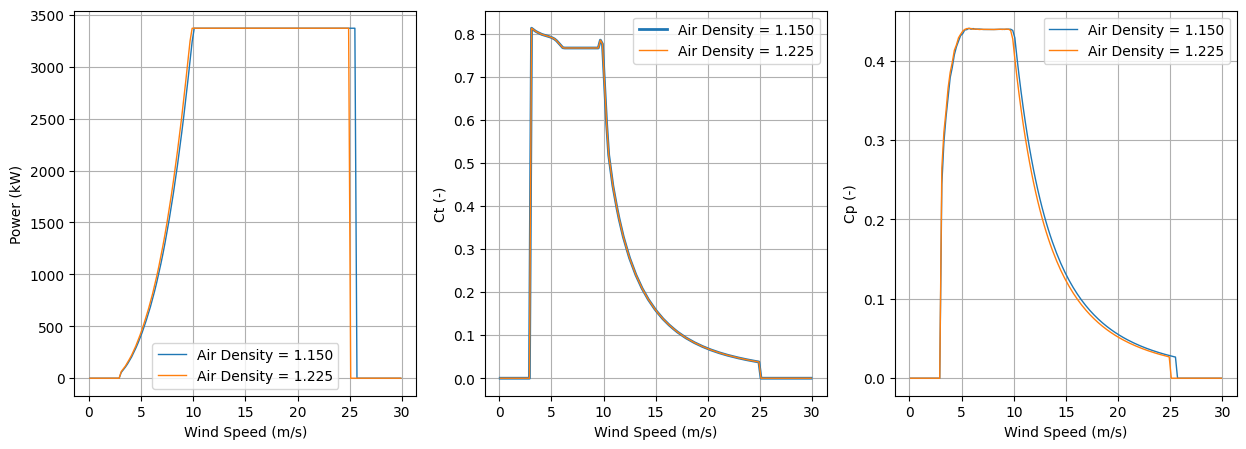
\includegraphics[width=0.92\linewidth]{Power Cp Ct.png}
		\caption{Turbine characteristic plots for power, $C_p$, and $C_t$ (from FLORIS and not from CSV).}
		\label{fig:power-cp-ct}
	\end{figure}
	
	\begin{figure}[h!]
		\centering
		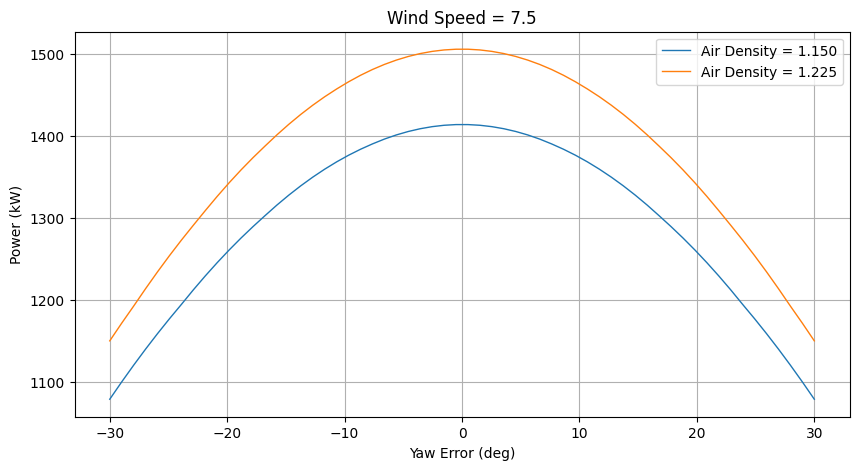
\includegraphics[width=0.92\linewidth]{Yaw Error.png}
		\caption{Power variation with yaw error in the range $[-30^\circ,30^\circ]$.}
		\label{fig:yaw-error}
	\end{figure}
	
	\subsection{Comment on the curve trend}
	The power values increase smoothly with wind speed until rated power is reached. This matches the expected control behavior of a pitch-regulated turbine. The $C_t$ and $C_p$ curves also follow the standard FLORIS turbine response.
	
	\section{Question 3: Visualize the wind farm flow field}
	The three-turbine farm was arranged in a straight line with turbine spacing of 5D. The flow field was visualized in three planes:
	\begin{itemize}[leftmargin=1.2em]
		\item horizontal plane at hub height,
		\item streamwise plane,
		\item spanwise plane.
	\end{itemize}
	
	The notebook created these views for two wind directions. In the notebook's coordinate setup, the aligned and wake-interaction cases were evaluated using 0$^\circ$ and 270$^\circ$.
	
	\subsection{Flow-field figures}
	\begin{figure}[h!]
		\centering
		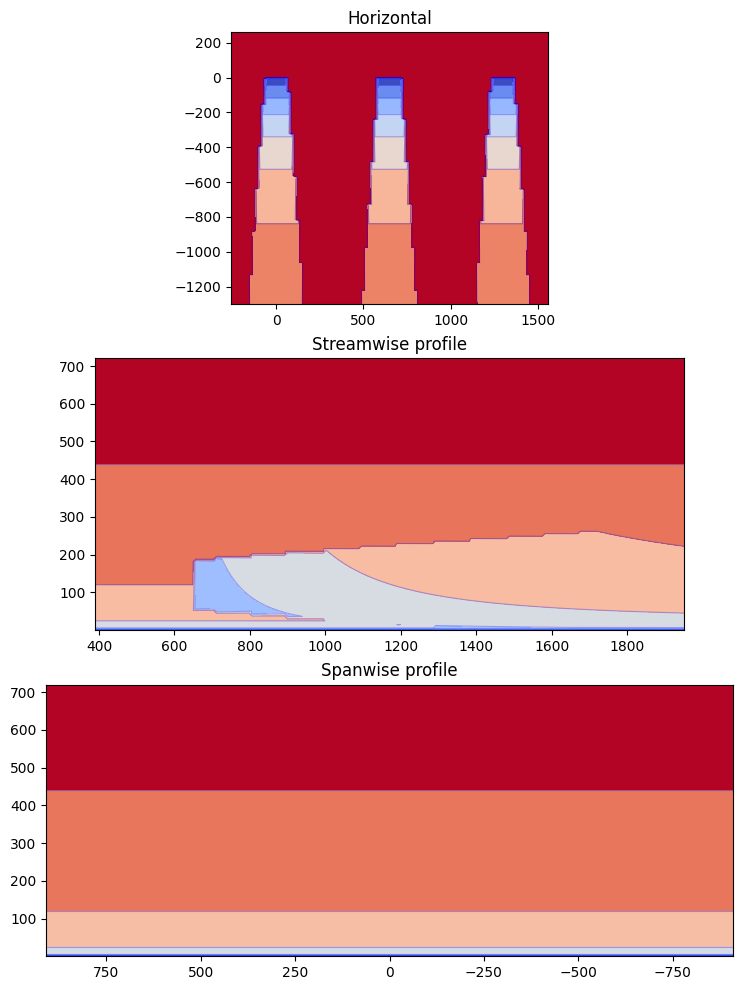
\includegraphics[width=0.8\linewidth]{Horizontal Streamvise CrossPlane 0Deg.png}
		\caption{Horizontal, streamwise, and cross-plane flow visualization for the 0$^\circ$ case.}
		\label{fig:flow-0deg}
	\end{figure}
	
	\begin{figure}[h!]
		\centering
		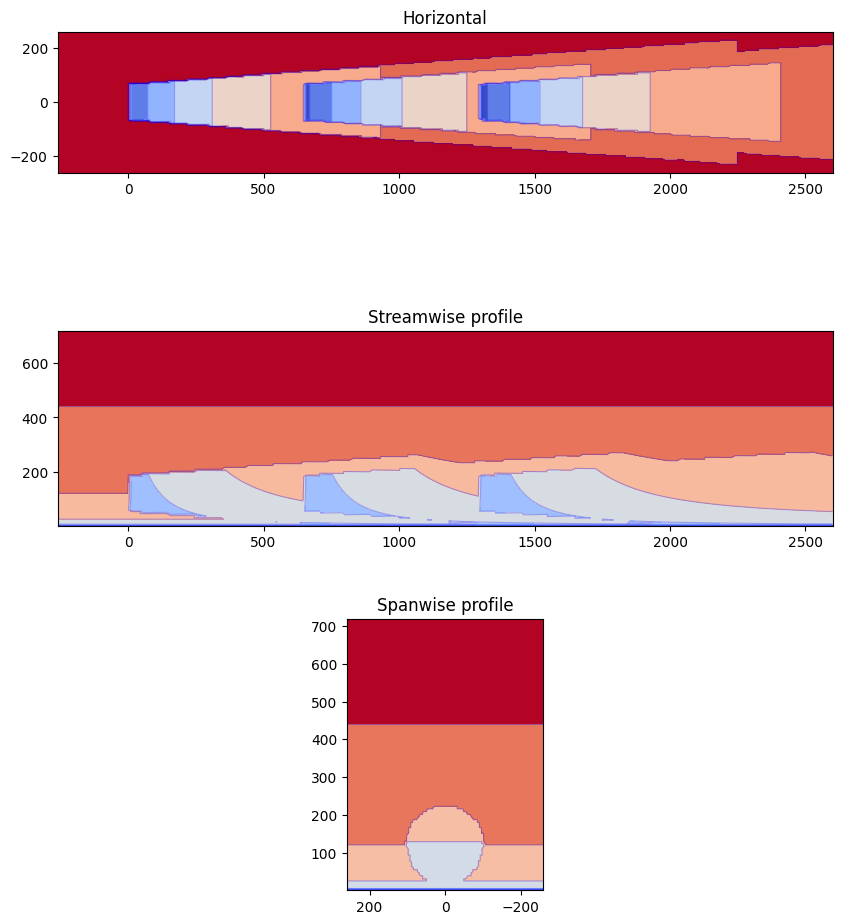
\includegraphics[width=0.8\linewidth]{Horizontal Streamvise CrossPlane 270Deg.png}
		\caption{Horizontal, streamwise, and cross-plane flow visualization for the 270$^\circ$ case.}
		\label{fig:flow-270deg}
	\end{figure}
	
	\subsection{Interpretation}
	The upstream turbine produces a wake deficit that is visible in the downstream flow field. In the aligned case, the wakes are narrow and clearly aligned with the turbine row. In the more oblique case, the wake footprint shifts across the farm, changing which downstream turbine is most affected. The spanwise and streamwise cuts help show wake expansion and velocity recovery away from the rotor plane.
	
	\section{Question 4: Jensen wake model power calculation}
	For the Jensen wake model with $k_w = 0.075$, the turbine and farm power were computed at 7.5 m/s for the two wind directions used in the notebook. The results were then compared with the hand calculations from Assignment 2.
	\newpage
	\subsection{Aligned / no-wake case}
	\begin{lstlisting}
		Absolute Power [kW]
		Floris               Hand Calculations   Error
		T1: 1505.9           T1: 1515.2          T1: 0.610%
		T2: 1505.9           T2: 1515.2          T2: 0.610%
		T3: 1505.9           T3: 1515.2          T3: 0.610%
		Farm: 4517.7         Farm: 4545.5        Farm: 0.610%
	\end{lstlisting}
	
	\newpage
	
	\subsection{Wake case}
	\begin{lstlisting}
		Absolute Power [kW]
		Floris               Hand Calculations   Error
		T1: 1505.9           T1: 1515.2          T1: 0.610%
		T2: 866.6            T2: 872.4          T2: 0.665%
		T3: 807.3            T3: 812.4          T3: 0.630%
		Farm: 3179.8         Farm: 3199.9        Farm: 0.630%
	\end{lstlisting}
	
	\subsection{Discussion}
	The FLORIS results are very close to the hand-calculated values from Assignment 2. The relative errors stay below 1\%, which is a strong indication that the model setup is consistent. A likely source of the small difference is that FLORIS uses numerical wake interaction and interpolated turbine characteristics, while the hand calculation is based on simplified analytical assumptions.
	
	\section{Question 5: Effect of increasing the spacing from 5D to 10D}
	The same Jensen wake setup was repeated for the aligned case and for the wake case, with turbine spacing increased from 5D to 10D.
	
	\subsection{Aligned case}
	\begin{lstlisting}
		Difference between 5D and 10D
		5D                  10D                 Relative Difference wrt 5D
		T1: 1505.9          T1: 1505.9          T1: 0.000%
		T2: 1505.9          T2: 1505.9          T2: 0.000%
		T3: 1505.9          T3: 1505.9          T3: 0.000%
		Farm: 4517.7        Farm: 4517.7        Farm: 0.000%
	\end{lstlisting}
	
	\subsection{Wake case}
	\begin{lstlisting}
		Difference between 5D and 10D
		5D                  10D                 Relative Difference wrt 5D
		T1: 1505.9          T1: 1505.9          T1: 0.000%
		T2: 866.6           T2: 1163.2          T2: 34.235%
		T3: 807.3           T3: 1140.5          T3: 41.272%
		Farm: 3179.8        Farm: 3809.6        Farm: 19.808%
	\end{lstlisting}
	
	\subsection{Discussion}
	Increasing the spacing from 5D to 10D gives the wake more distance to recover before reaching the next turbine. As a result, downstream turbines experience a higher inflow velocity and therefore generate more power. The farm power rises noticeably in the wake case, which is exactly the expected physical trend.
	
	\section{Question 6: Day and night conditions with Gaussian wake model}
	The Gaussian wake model was used to study how atmospheric stability changes affect power generation. Two conditions were tested:
	\begin{itemize}[leftmargin=1.2em]
		\item \textbf{Day}: wind shear exponent 0.06, turbulence intensity 12\%.
		\item \textbf{Night}: wind shear exponent 0.22, turbulence intensity 6\%.
	\end{itemize}
	
	\subsection{5D spacing, wind direction 0$^\circ$}
	\begin{lstlisting}
		Day               Night             Increase/Decrease in Power
		T1: 1509.5        T1: 1506.7        T1: -0.186%
		T2: 1509.5        T2: 1506.7        T2: -0.186%
		T3: 1509.5        T3: 1506.7        T3: -0.186%
	\end{lstlisting}
	
	\subsection{5D spacing, wake-aligned case}
	\begin{lstlisting}
		Day               Night             Increase/Decrease in Power
		T1: 1509.5        T1: 1506.7        T1: -0.186%
		T2: 725.0         T2: 396.6         T2: -82.824%
		T3: 760.6         T3: 464.8         T3: -63.659%
	\end{lstlisting}
	
	As observed above, the wake of Turbine T1 causes a significant drop in produced turbine power in Turbine T2. The lower turbine power produced by T2 due to wake from T1 causes lower wake of T2 on T3, the wake from T1 is also reduced due to the distance as well as interference from T2. This sees an increase in turbine power of T3 when compared to T2.
	
	\subsection{20D spacing, wake-aligned case}
	\begin{lstlisting}
		Day         Night           Increase/Decrease in Power
		T1: 1509.5  T1: 1506.7      T1: -0.186%
		T2: 1366.1  T2: 1172.9      T2: -16.465%
		T3: 1360.1  T3: 1155.5      T3: -17.707%
	\end{lstlisting}
	
	As the inter-turbine distance is increased to 20*Rotor Diameter, the dip of turbine power of T2 is seen to be gone.
	
	\subsection{Discussion}
	The day case has higher turbulence intensity, which promotes faster wake mixing and faster recovery of downstream flow. The night case has lower turbulence intensity, so the wakes remain stronger for longer and the downstream turbines lose more power. The higher wind shear at night also changes the vertical inflow profile, which can further modify the wake structure. In the 10D layout, the wakes have more space to recover, so the downstream turbines perform much better than in the 5D case.
	
	\subsection{Flow-field interpretation}
	The visualizations for day and night show the same overall wake pattern, but the wake deficit is stronger and persists farther downstream at night. This is consistent with lower turbulence intensity and reduced wake diffusion. During the day, enhanced mixing helps the wake recover sooner, so the velocity deficit behind each turbine becomes smaller.
	
	\section{Conclusion}
	This assignment showed how to define a custom wind turbine in FLORIS, validate its performance curves, visualize flow fields, and compare wake-model predictions for different spacings and atmospheric conditions. The main conclusions are:
	\begin{itemize}[leftmargin=1.2em]
		\item the turbine curve setup is consistent with the provided IEA 3.4 MW data,
		\item FLORIS results match the hand calculations closely,
		\item larger turbine spacing reduces wake losses,
		\item higher turbulence intensity improves wake recovery and raises downstream power production.
	\end{itemize}
	
\end{document}


